%%%%%%%%%%%%%%%%%%%%%%%%%%%%%%%%%%%%%%%%%
% University/School Laboratory Report
% LaTeX Template
% Version 3.1 (25/3/14)
%
% This template has been downloaded from:
% http://www.LaTeXTemplates.com
%
% Original author:
% Linux and Unix Users Group at Virginia Tech Wiki 
% (https://vtluug.org/wiki/Example_LaTeX_chem_lab_report)
%
% License:
% CC BY-NC-SA 3.0 (http://creativecommons.org/licenses/by-nc-sa/3.0/)
%
%%%%%%%%%%%%%%%%%%%%%%%%%%%%%%%%%%%%%%%%%

%----------------------------------------------------------------------------------------
%	PACKAGES AND DOCUMENT CONFIGURATIONS
%----------------------------------------------------------------------------------------

\documentclass{article}

\usepackage[version=3]{mhchem} % Package for chemical equation typesetting
\usepackage{siunitx} % Provides the \SI{}{} and \si{} command for typesetting SI units
\usepackage{graphicx} % Required for the inclusion of images
\usepackage{natbib} % Required to change bibliography style to APA
\usepackage{amsmath} % Required for some math elements 
\usepackage[utf8]{inputenc}
\usepackage{tikz,pgfplots}
\usepackage[letterpaper, margin=0.5in]{geometry}
\usepackage{float}
\usepackage{enumitem}
\usepackage{fixltx2e}
\usepackage{gensymb}
\usepackage[hidelinks]{hyperref}
\usepackage[all]{hypcap}

\usepackage{xcolor}

% Roman numerials
\pagenumbering{arabic}

\setlength\parindent{0pt} % Removes all indentation from paragraphs

%\renewcommand{\labelenumi}{\alph{enumi}.} % Make numbering in the enumerate environment by letter rather than number (e.g. section 6)

%\usepackage{times} % Uncomment to use the Times New Roman font

% for some tables
\newcommand{\specialcell}[2][c]{%
  \begin{tabular}[#1]{@{}c@{}}#2\end{tabular}}
  
\providecommand{\e}[1]{\ensuremath{\times 10^{#1}}}
%----------------------------------------------------------------------------------------
%	DOCUMENT INFORMATION
%----------------------------------------------------------------------------------------

%\title{Determination of the Atomic \\ Weight of Magnesium \\ CHEM 101} % Title

%\author{John \textsc{Smith}} % Author name

%\date{\today} % Date for the report

\begin{document}

%\maketitle % Insert the title, author and date

% If you wish to include an abstract, uncomment the lines below
% \begin{abstract}
% Abstract text
% \end{abstract}

%----------------------------------------------------------------------------------------
%	SECTION 1
%----------------------------------------------------------------------------------------

\section{Objective}

To determine the percent weight of Sb in an unknown Pb-Sb alloy using two techniques. The first being generating a cooling curve for our sample and comparing it with the Pb-Sb phase diagram as well as cooling curves for various values of \% w Sb in Pb in order to generate field boundary temperatures for our sample. Second, we create a mold of the sample and view the microstructure under a microscope to view the solidus material and decide wheather the sample was in the hypoeutectic, eutectic, or hypereutectic regions.

% If you have more than one objective, uncomment the below:
%\begin{description}
%\item[First Objective] \hfill \\
%Objective 1 text
%\item[Second Objective] \hfill \\
%Objective 2 text
%\end{description}

%----------------------------------------------------------------------------------------
%	SECTION 2
%----------------------------------------------------------------------------------------

\section{Experimental Procedures}
\subsection{Pre Lab}
Before coming into lab, we made sure to understand the following cooling curves for lead-antimony.
\begin{figure}[H]
\centering
\begin{tikzpicture}
\node at (0,0) {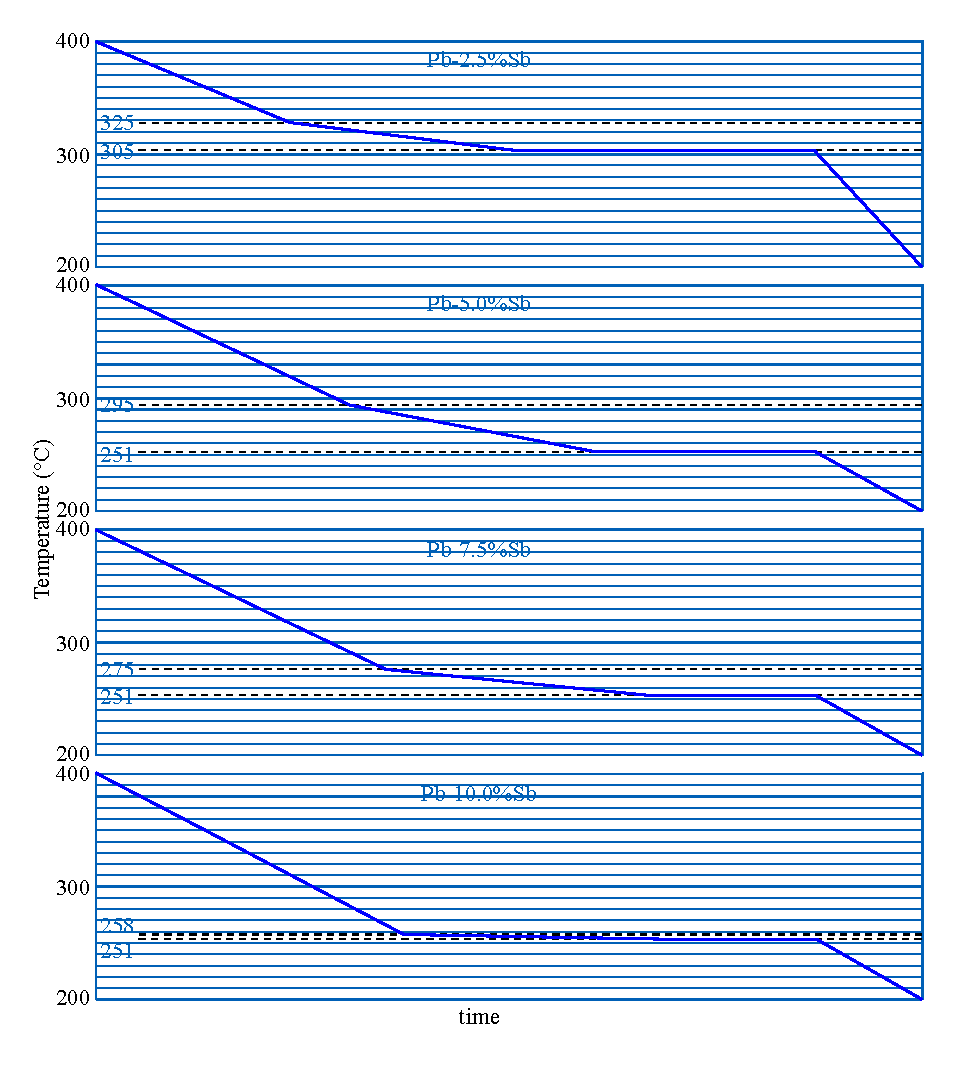
\includegraphics[width=250pt]{pics/diagram1.pdf}};
\node at (10,0) {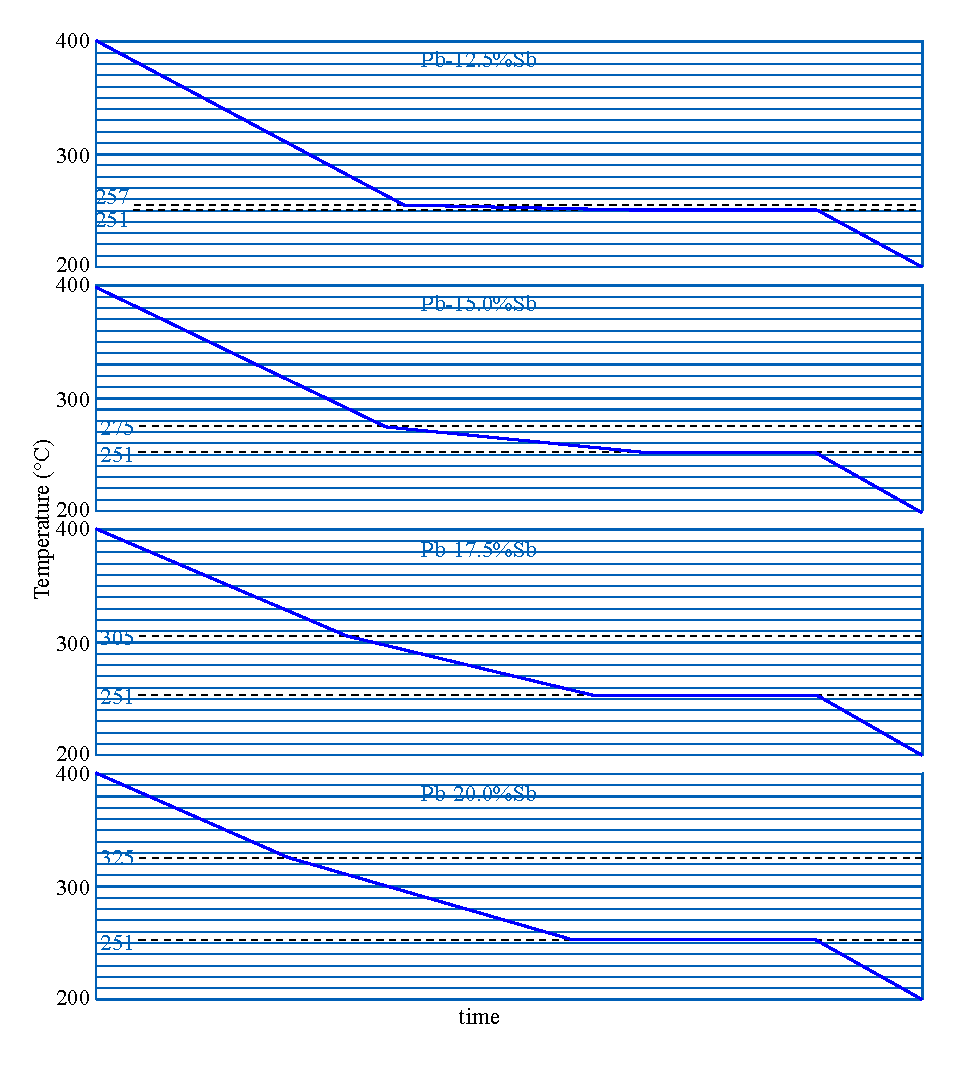
\includegraphics[width=250pt]{pics/diagram2.pdf}};
\end{tikzpicture}
\caption{Cooling curves for various \% antimony (Sb) in lead (Pb). Note the slope changes that occur at various temperatures where phase change occurs. To see in detail, just zoom into figure. [2]}
\label{fig:ccoriginal}
\end{figure}
We compared these various cooling curves with the phase diagram for Pb-Sb.
\begin{figure}[H]
\centering
\begin{tikzpicture}
\node at (0,0) {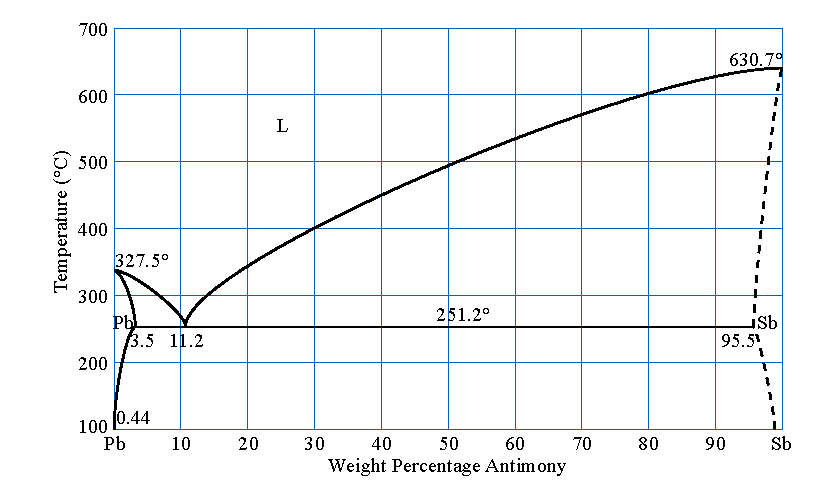
\includegraphics[width=300pt]{pics/diagram.pdf}};
\draw [dotted,red,thick] (-3.3,-2.7) -- (-3.3,3);
\draw [dotted,red,thick] (-2.85,-2.7) -- (-2.85,3);
\draw [dotted,red,thick] (-2.5,-2.7) -- (-2.5,3);
\node at (-3.4,-2.8) {5\%};
\node at (-2.4,-2.8) {15\%};
\end{tikzpicture}
\caption{Phase diagram for Pb-Sb. The 3 dotted lines represent the \% Sb available for the lab. [2]}
\end{figure}
\label{fig:phased}
For the lab three different vials were available. These vials contained either 5\%, 11.2\%, or 15\% Sb. Note the 11.2 \% is at the eutectic point. Understanding figure 1 was crucial for helping us figure out which sample we had for our group.

\subsection{Cooling Curves}
First we recorded the \# on our sample (3). Next we plugged the vial with a 'lava plug'. We placed a glass thermocouple sleeve through the top of the lava plug into the vial. Next we placed a brass stop collar over the thermocouple sleeve and left about a 0.5 inch gap between the brass collar and the top of the lava plug where the therocouple sleve enters the vial. Finally we placed the thermocouple through the thermocouple sleeve and connected the thermocouple to the data acquisition interface. Refer to figure 3 for a complete set up.
\begin{figure}[H]
\centering
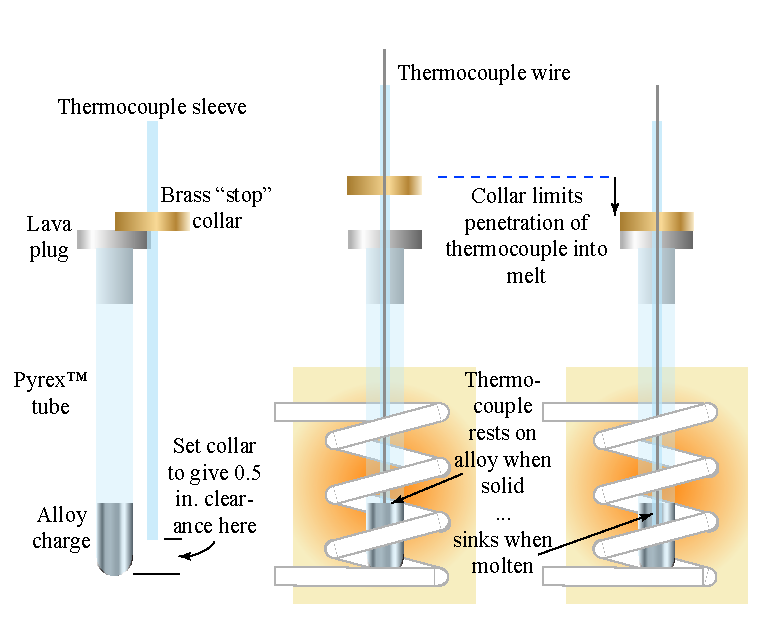
\includegraphics[width=300pt]{pics/diagram3.pdf}
\caption{Schematic showing experimental set-up for determining cooling curves. A small gap at the bottom of the Pyrex tube assures that the thermocouple is reading the temperature of the alloy and not the glass containment vessel. The gap is measured as shown at the left. After melting, the thermocouple sinks into position, as shown on the right. [2]}
\label{fig:diagram}
\end{figure}

We then turned on the furnace power and started heating the sample. At the same time we turned on out data acquisition program to start recording temperature as a function of time. At around 280$\degree$C we slowed down the furnace power in order to hit the target temperature of 300$\degree$C. As the alloy started to melt, we observed our brass stop collar fall and make contact with the lava stopper. When the temperature hit about 305$\degree$C we turned off the heating furnace and had the sample cool back down to about 200$\degree$C.

\subsection{Sample Acquisition}
Now that the sample has cooled to about 200$\degree$C and we have cooling curves, we heated the sample back up to the melting point temperature of 360$\degree$C. At the same time we turned on the Al mold heating by setting the target temperature to 280$\degree$C. Make sure to have another thermocouple inserted into the small hole on the side of the Al mold to record the temperature. The Al mold heating device should take the temperature of the mold up to 280$\degree$C and keep it constant at that temperature. Once the Al mold reaches 280$\degree$C and the vial with the sample reaches 360$\degree$C we prepared for the transition. 

Quickly remove the thermocouple, thermocouple sleeve, brass collar, and lava plug from the sample vial. Try to avoid getting injured here as everything is still very hot. Now we used the tongs to quickly and safely remove the sample vial from the heating furnace and pour the liquid sample into the hole ontop of the Al mold device. Make sure to remove the thermocouple that was put into the Al mold before pouring! Once the sample is poured, we set the temperature to 0$\degree$C for the Al mold and turned off the heating furnace the sample was originally in. Once the Al mold had cooled, we twisted the two knobs on the back of the device and push the lever on the right side of the device to release the mold container. We used the tongs to grab the mold and drop it in a sink full of water to further cool the device. The lab GSI then extracted our sample from the mold using a drill and hammer. Finally we etched the surface of our sample with some nitric acid before heading into the microscope room to make observations.

%----------------------------------------------------------------------------------------
%	SECTION 3
%----------------------------------------------------------------------------------------
\section{Experimental Results}
\begin{figure}[H]
\centering
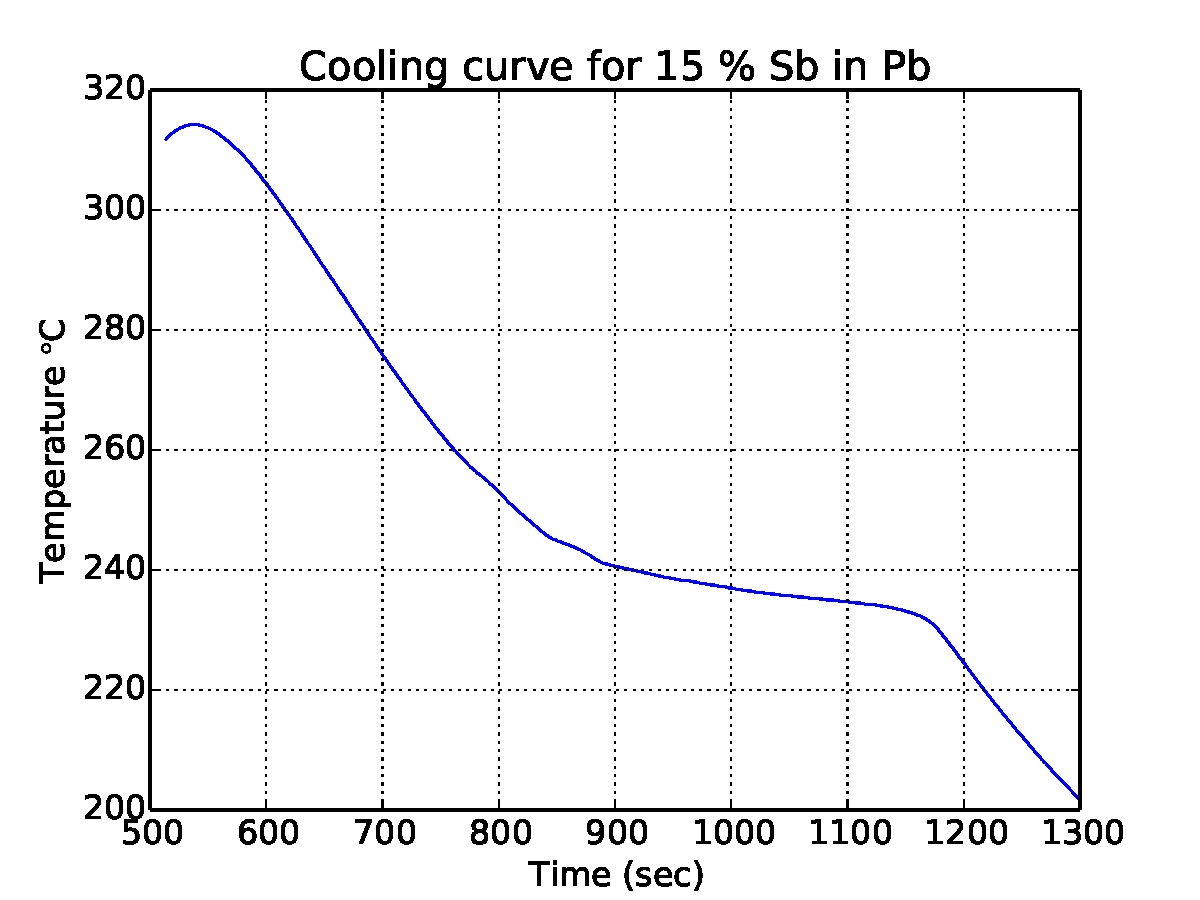
\includegraphics[width=350pt]{graphs/graph1.pdf}
\caption{Cooling curve for 15\% Sb in Pb. Note how there is no distinct change in the slope at the 240$\degree$C line.}
\label{fig:cc}
\end{figure}

\section{Experimental Results}
\begin{figure}[H]
\centering
\begin{tikzpicture}
\node at (0,5) {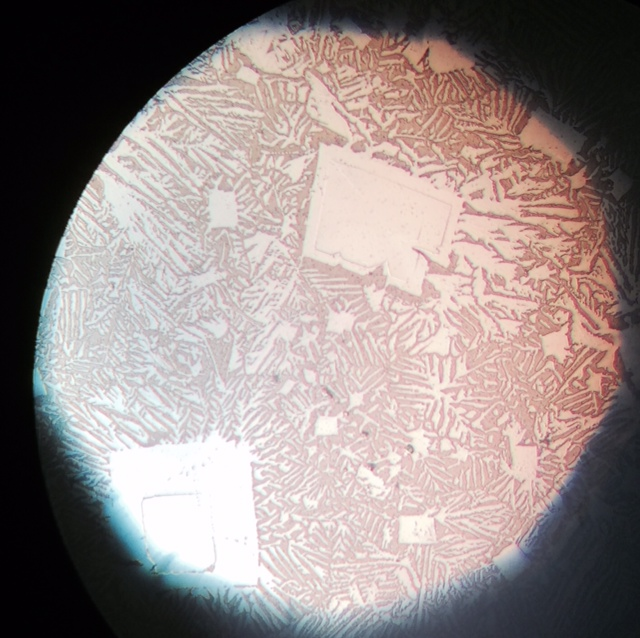
\includegraphics[height=270pt]{pics/image2.jpeg}};
\node at (10,5) {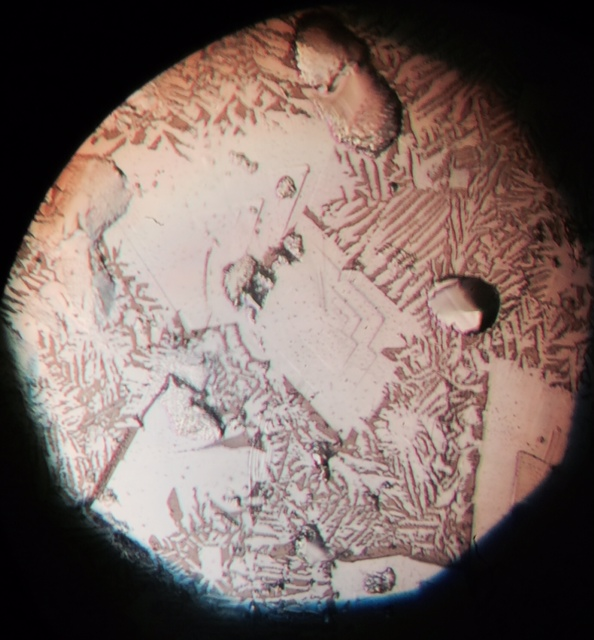
\includegraphics[height=270pt]{pics/image3.jpeg}};
\end{tikzpicture}
\caption{Note the big solid squares of Sb that formed in the Sb + L phase. Also the lamellae that formed later when the sample cooled into the solid Pb + Sb phase. The image on the right is a magnification. Note the various layers of solid Pb in the picture on the right.}
\label{fig:images}
\end{figure}

\section{Discussion}

\begin{description}[style = nextline]
\item[1) By direct comparison of your cooling curves and the phase diagram, what can you conclude about the composition of your alloy? How confident are you? Explain your answer in detail, noting all sources of experimental error and what you did to minimize them. What might you do to improve precision? Accuracy?]

Looking at the cooling curve we generated (Fig \textcolor{blue}{\ref{fig:cc}}), it is hard to distinguish two different slopes; this makes us believe that it must be either 11.2 \% or 15 \% Sb, eliminating the possibility of it being 5 \% Sb since this has two very distinct slope changes. Noting that our temperature for our cooling curve is no where close to the phase transition temperatures present on the cooling curves in Fig \textcolor{blue}{\ref{fig:ccoriginal}}, this makes it hard to figure out what composition we have. However, after viewing the images under the microscope, it is very obvious that our sample is in the hypereutectic region. The microscope images show solid pieces of Sb which must have formed in the Sb + L phase as well as a lot of lamellae which can have only formed once we were in the solid Sb + Pb phase. 

The biggest problems and experimental error we ran into was the temperature measurements. The temperature at which we made our transistion between phases was about 240$\degree$C, but the theoretical temperature transistion into the Sb + L phase should have occured at 275$\degree$C for 15\% Sb. Most likely our thermocouple was placed wrong in such a way that it measured our data with a 20$\degree$C offset. Another possibility is that the cold junction reference temperature of 0$\degree$C for the thermocouple was not set up correctly; this would explain our ~20$\degree$C offset in the data.

To improve accuracy, we could make sure our thermocouple is in the correct position and measuring the temperature of the sample. For precision there should be a better method for transitioning from the furnace heating element to the Al mold. Maybe if we had better glassware that allowed us to heat up the sample to higher temperatures, we could improve the chance of the sample hardening before it goes into the Al mold.
\label{description}

\item[2)Describe the successive changes in microstructure that took place during solidification of your alloy.  Write a detailed caption for your sketch of the microstructure from your specimen. Label the microconstituents seen in your sketch and give your opinion of both the composition and the temperature at which each constituent solidified. Comment specifically on how you identified the Pb-rich constituent, the Sb-rich constituent, and the eutectic constituent.  Cite all relevant references to support your answers.]

Looking at the phase diagram in Fig \textcolor{blue}{\ref{fig:phased}} we can see what phases our sample went through by looking at the dotted 15 \% Sb red line. At around 360$\degree$C our sample is in an all liquid phase. At somewhere around the 320 line our sample begins to transistion into the Sb + L phase. The sample now starts nucleating. Between 320$\degree$C and 251$\degree$C we are in the Sb + L phase and the antimony in the sample starts solidifying into square and triangle like shapes. while the rest of the sample remains a liquid. Once we reach the eutectic temperature of 251$\degree$C we transition into the Pb + Sb solid phase. This means that all the liquid should be gone and replaced by a microstruture of alternating lamellae. However, the solid Sb that formed in the Sb + L phase should still remain as well. So in the end we will have large solids of Sb that formed in the previous Sb + L phase as well as a lot of lamellae, which are alternating strips of solid Sb and Pb, that formed after we passed the Eutectic temperature transforming all the liquid into solid Sb + Pb.
\begin{figure}[H]
\centering
\begin{tikzpicture}
\node at (0,5) {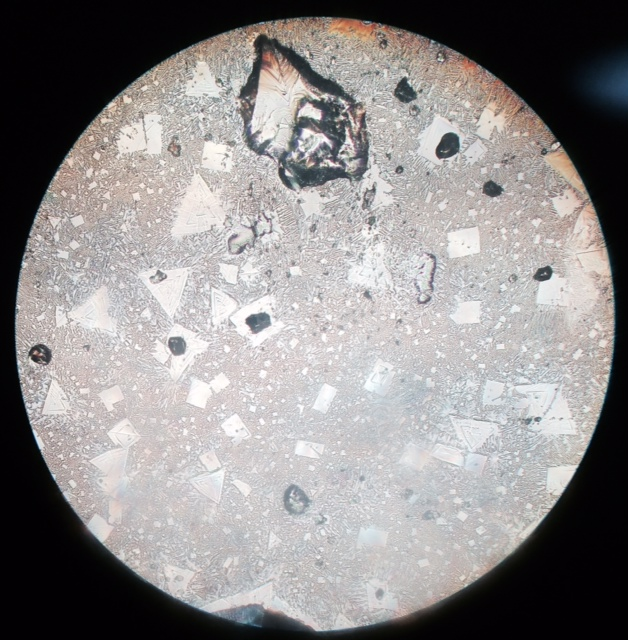
\includegraphics[height=250pt]{pics/image1.jpeg}};
\node at (10,5) {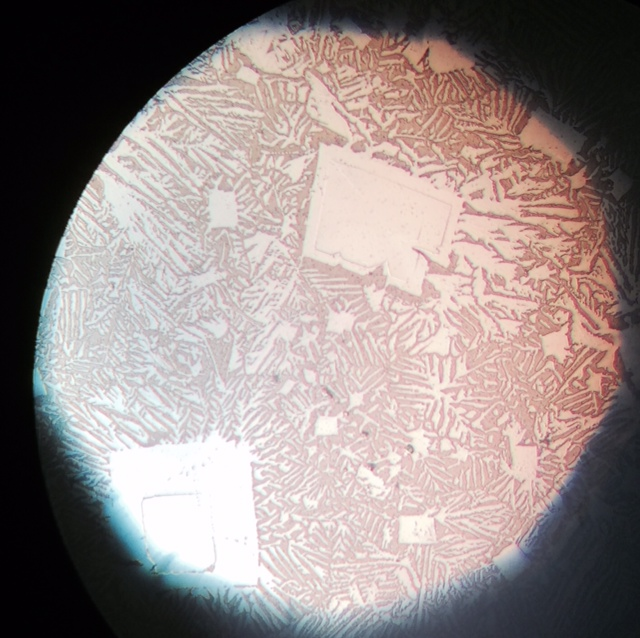
\includegraphics[height=250pt]{pics/image2.jpeg}};
\node at (-1.5,6.5) {\color{red}{*}};
\node at (-2,5.4) {\color{red}{*}};
\node at (-1.55,3.9) {\color{red}{*}};
\node at (3.3,3.6) {\color{red}{*}};
\node at (2,6) {\color{red}{*}};
\draw [thick,blue] (0.3,4.8) circle [radius=5pt];
\draw [thick,blue] (0.3,4.6) -- (10,1.5);
\draw [thick,blue] (0.3,5) -- (10,8.5);
\draw [thick,blue] (10,5) circle [radius=100pt];
\draw [thick,blue] (9,4) circle [radius=10pt];
\draw [thick,blue] (11.5,4) circle [radius=10pt];
\node at (11,6.4) {\color{red}{*}};
\node at (8,2) {\color{red}{*}};
\draw [black] (0,-2) rectangle (10,-0);
\node at (4.3,-0.5) {\color{red}{*} Various solidified Sb that formed in Sb + L phase};
\node at (4.8,-1.5) {\color{blue}{$\circ$} Example of alternating lamellae formed in Sb + Pb phase};
\end{tikzpicture}
\caption{Image on the right is a magnified image of the structure from the left. The large solid pieces of Pb were formed in the Sb + L phase which is between ~320$\degree$C and 251$\degree$C. The rest of the solid is filled with lamellae which formed after we hit temperatures below 251$\degree$C meaning we transitioned into the Pb + Sb phase. Noting that the eutectic point is very close the the Pb phase and using the phase rule, we can see that the majority of the lamellae should be Pb. }
\label{fig:que2}
\end{figure}

\end{description}

%----------------------------------------------------------------------------------------
%	SECTION 4
%----------------------------------------------------------------------------------------

\section{Conclusions}
As a result of this investigation, the following conclusions can be drawn.
\begin{enumerate}
\item The sample we were given contains approximately 15 \% w Sb in Pb.
\item The cooling curve generated matches closest with the cooling curve for 10-15 \% w Sb in Pb.
\item The temperature in the cooling curve generated remains relatively constant when hitting the melting temperature.
\item The microstructure definitely contains solid pieces of Sb which can only have formed in the Sb + L phase, the hypereuctectic region.
\item The microstructure also contains lamellae which formed in the Pb + Sb phase. \\*[2cm]
\end{enumerate}

%----------------------------------------------------------------------------------------
%	SECTION 5
%----------------------------------------------------------------------------------------

\section{References}
\begin{enumerate}
\item James F. Shackelford, Introduction to Materials Science for Engineers, Seventh Edition, Pearson Higher 
Education, Inc., Upper Saddle River, New Jersey (2009).
\item Gronsky, Ron. Lab 04 Manual: Binary Alloy Phase Diagrams. Berkeley: Ronald Gronsky, 2014. Web.
\end{enumerate}

%----------------------------------------------------------------------------------------
%	SECTION 6
%----------------------------------------------------------------------------------------

% Nothing right now

%----------------------------------------------------------------------------------------
%	BIBLIOGRAPHY
%----------------------------------------------------------------------------------------

\bibliographystyle{apalike}

\bibliography{sample}

%----------------------------------------------------------------------------------------


\end{document}

